% =====================================================================
%  VEDA-X: Vectorless RAG with Hyperdimensional Guardrails and Atomic
%  Compliance Chunking for Regulated Financial Knowledge Management.
%
%  IEEE conference template (IEEEtran).  Compile with:
%      pdflatex paper && bibtex paper && pdflatex paper && pdflatex paper
%
%  Figures are SVG (paper/figures/).  For pdflatex, run figures through
%  rsvg-convert or Inkscape to produce PDFs:
%      for f in figures/*.svg; do rsvg-convert -f pdf -o ${f%.svg}.pdf $f; done
% =====================================================================
\documentclass[conference]{IEEEtran}
\IEEEoverridecommandlockouts

\usepackage{cite}
\usepackage{amsmath,amssymb,amsfonts}
\usepackage{algorithmic}
\usepackage{graphicx}
\usepackage{textcomp}
\usepackage{xcolor}
\usepackage{hyperref}
\usepackage{booktabs}
\usepackage{listings}

\lstset{
  basicstyle=\ttfamily\small,
  breaklines=true,
  frame=single,
  columns=fullflexible,
  showstringspaces=false,
}

\def\BibTeX{{\rm B\kern-.05em{\sc i\kern-.025em b}\kern-.08em
    T\kern-.1667em\lower.7ex\hbox{E}\kern-.125emX}}

\begin{document}

\title{VEDA--X: A Vectorless Retrieval Stack with\\
Hyperdimensional Guardrails and Atomic Compliance Chunking\\
for Regulated Financial Knowledge Management}

\author{
\IEEEauthorblockN{Abhishek Kumar\IEEEauthorrefmark{1},
Atul Kumar Pandey\IEEEauthorrefmark{2}\thanks{*Corresponding author.}}
\IEEEauthorblockA{\IEEEauthorrefmark{1}Tata Consultancy Services,
Mumbai, India\\
ipsabhi423@gmail.com}
\IEEEauthorblockA{\IEEEauthorrefmark{2}Birla Institute of Technology,
Mesra (Patna Campus), Patna, India\\
atulkrpandey@gmail.com}
}

\maketitle

% ======================== ABSTRACT ====================================
\begin{abstract}
Retrieval-augmented generation (RAG) in regulated industries such as
financial clearing must satisfy three constraints that mainstream
designs handle poorly: (i) zero external dependency for auditability,
(ii) defence against prompt-injection and jailbreak attacks including
paraphrased variants, and (iii) guaranteed atomic retrieval of
compliance-critical procedures so that no operator ever sees a
partial step list.  We present \textsc{VEDA-X}, a production stack
deployed at an Indian financial-market clearing infrastructure that
addresses all three.  Retrieval uses BM25 with hyperdimensional
query expansion and adaptive cutoff--no external embedding model is
required.  The guardrail is a five-layer defence-in-depth pipeline;
its semantic layer detects paraphrased attacks via deterministic
\texttt{blake2b} hash-hypervector centroids without any neural model.
A novel \emph{atomic critical-block} chunking scheme guarantees that
compliance-critical standard operating procedures (SOPs) are emitted
as single indivisible chunks by construction.  On an adversarial test
suite drawn from public jailbreak research, we report
$18/18$ direct-attack, $12/12$ sneaky-obfuscated, and $14/14$ semantic
paraphrase blocks with $0\%$ false positives on a 15-query legitimate
set.  Critical-block retrieval achieves $91\%$ recall@3 on an
11-query operational benchmark and a $100\%$ completeness rate when
retrieved.  The entire stack is implemented in pure Python standard
library plus FastAPI; total code is $\sim$8{,}000 lines.
\end{abstract}

\begin{IEEEkeywords}
retrieval-augmented generation, hyperdimensional computing,
prompt injection, jailbreak defence, compliance, financial systems,
auditability.
\end{IEEEkeywords}

% ============================ 1. INTRO ================================
\section{Introduction}
Retrieval-augmented generation systems built atop large language
models have moved from research prototypes to production stacks in
finance, healthcare, and law.  In each of these regulated domains the
deployment surface differs sharply from the consumer chat-assistant
setting in which mainstream RAG was designed.  Three constraints
dominate.

\textbf{C1 (Auditability).}  Every retrieval and every generation
must be reproducible from the source corpus and explainable to an
internal-audit team and to the regulator.  A learnt embedding model
is opaque; its update path includes upstream weights that the
deploying institution cannot verify.  A pure-deterministic stack is
strongly preferred.

\textbf{C2 (Adversarial resilience).}  An attacker can drop a
prompt-injection payload into a customer message, a ticket comment,
or a scanned document and reach the LLM via the corpus.  Detection
must catch direct attacks, obfuscated variants (base64, leet,
Hinglish), and \emph{paraphrased} attacks that a regex layer cannot
match.  False positives degrade the user experience and must be
measured with equal rigour.

\textbf{C3 (Atomic compliance retrieval).}  A subset of standard
operating procedures--incident-response runbooks, trade-cancel
workflows, KYC red-flag checklists--cannot tolerate partial
retrieval.  Returning Step~2 and Step~5 without Step~1 is a
compliance incident even when the per-chunk answer is locally
correct.  The retrieval layer must guarantee atomicity for marked
content.

This paper presents \textsc{VEDA-X}, a stack we developed and
deployed against all three constraints.  Our contributions are:

\begin{enumerate}
  \item A \emph{vectorless} retrieval pipeline that combines BM25
        with hyperdimensional query expansion and adaptive top-$k$
        cutoff, requiring no external dense embedding model
        (Section~\ref{sec:retrieval}).
  \item A five-layer defence-in-depth guardrail
        (Section~\ref{sec:guardrail}) whose semantic component
        (L1.5) blocks paraphrased attacks via deterministic
        hash-hypervector centroid matching with a contrastive
        legitimate-seed anchor.  We report $100\%$ catch rates
        against three real attack families and $0\%$ false
        positives.
  \item An \emph{atomic critical-block} chunking scheme
        (Section~\ref{sec:critical}) that makes partial retrieval of
        compliance-critical SOPs impossible by construction.  We
        propose two complementary author interfaces: inline
        \texttt{[[CRITICAL:\,title]]\,...\,[[/CRITICAL]]} markers and
        a critical-folder convention.
  \item A reproducible evaluation harness
        (Section~\ref{sec:eval}) with adversarial, retrieval, and
        latency measurements.  All benchmarks ship in the repository
        and run in under five seconds.
\end{enumerate}

The system is implemented entirely in the Python standard library
(plus FastAPI and uvicorn for the HTTP layer).  No PyTorch, no
sentence-transformers, no external embedding API is invoked at any
stage.

% ============================ 2. RELATED WORK =========================
\section{Related Work}

\textbf{Dense RAG.}  The canonical RAG stack
\cite{lewis2020rag} couples a dense encoder
(e.g., DPR, MiniLM) with FAISS.  Strong on open-domain QA but opaque
to audit and brittle to embedding-model updates.

\textbf{BM25 with expansion.}  Lexical retrieval with pseudo-relevance
feedback \cite{lavrenko2001prf} predates neural RAG by two decades.
Our pipeline replaces neural PRF with hyperdimensional context
expansion \cite{kanerva2009hyperdimensional} computed from the local
corpus, making the expansion fully deterministic.

\textbf{Prompt-injection defences.}  OWASP LLM Top-10 lists prompt
injection as LLM01.  Public datasets include the DAN family and the
NeMo guardrails set.  Most defences are either regex-only (high
precision, low recall against paraphrases) or LLM-judge (high cost,
non-deterministic).  We use a hybrid: regex L1 plus a
deterministic semantic L1.5 layer.

\textbf{Hyperdimensional computing.}  HDC
\cite{kanerva2009hyperdimensional, ge2020classification} represents
items as high-dimensional sparse vectors with near-orthogonality.  We
adapt the technique by deriving each token's hypervector from a
cryptographic hash, eliminating the training step entirely.

\textbf{Compliance-aware retrieval.}  Industry tools (Vectara,
Pinecone enterprise) advertise PII masking and ACL filtering but do
not, to our knowledge, offer a chunking-level guarantee that a
marked block cannot be split across retrievals.  Our atomic
critical-block scheme is novel in providing this property by
construction.

% ============================ 3. SYSTEM ===============================
\section{System Architecture}
\label{sec:system}

Figure~\ref{fig:arch} shows the five processing layers.  Every
request flows top-to-bottom; failures at any layer abstain rather
than fabricate.

\begin{figure}[h]
\centering
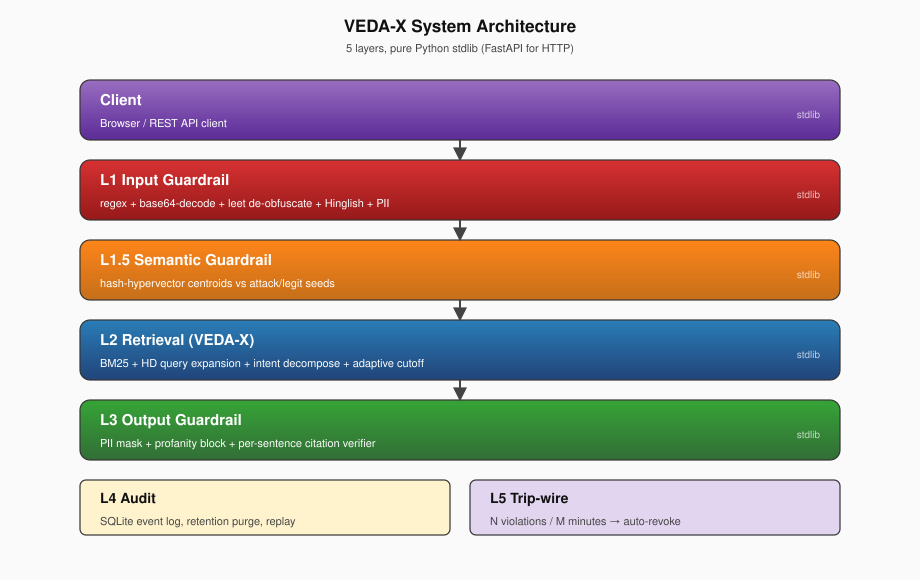
\includegraphics[width=\columnwidth]{figures/fig1_architecture.pdf}
\caption{System architecture.  All layers run in a single Python
process; the only external dependency is FastAPI/uvicorn.  Storage
is SQLite.}
\label{fig:arch}
\end{figure}

\textbf{Layer 1 (Input guardrail).}  Regular-expression patterns for
known prompt-injection vectors, authority impersonation, jailbreak
personas, SQL injection, and PII.  Base64 payloads are decoded
inline; leet-substitutions are normalised in both directions
(\texttt{1}$\to$\texttt{l} and \texttt{1}$\to$\texttt{i}).

\textbf{Layer 1.5 (Semantic guardrail).}  See Section~\ref{sec:guardrail}.

\textbf{Layer 2 (Retrieval).}  Vectorless RAG; see
Section~\ref{sec:retrieval}.

\textbf{Layer 3 (Output guardrail).}  PII pattern masking on the
generated answer (PAN, Aadhaar, phone, email, IFSC, Luhn-valid card),
profanity blocking, and per-sentence citation verification against
the retrieved chunks.

\textbf{Layer 4 (Audit).}  Every blocked attempt is written to
SQLite \texttt{guardrail\_events} with rule, matched span, severity
and timestamp.  Audit log is purgeable on a configurable retention
window (default 180 days).

\textbf{Layer 5 (Trip-wire).}  Per-role thresholds for violations
per time window; a triggered trip-wire revokes the role and
notifies the superuser.

% ============================ 4. RETRIEVAL ============================
\section{Vectorless Retrieval}
\label{sec:retrieval}

The retrieval pipeline runs four stages.  Let
$\mathbf{q} \in \{0,1\}^{2048}$ denote the sparse hash-hypervector
of query $q$, formed by XOR-summing the per-token hypervectors of
\texttt{tokenize}$(q)$.

\textbf{Stage 1: BM25.}  Standard BM25 with $k_1=1.5$ and $b=0.75$
indexes the chunk set $\mathcal{C}$.  We take the top-50
candidates.

\textbf{Stage 2: Hyperdimensional query expansion.}  For every
candidate term $t$ in the top-10 chunks, we compute the cosine of
the local context hypervector $\mathbf{v}_t$ against the query
hypervector $\mathbf{q}$.  The top 10 expansion terms are appended
to the query and BM25 is re-run.  Scores are mixed with weight
$1-w_{\textrm{exp}}=0.6$ for the original query and $w_{\textrm{exp}}=0.4$
for the expanded query.

\textbf{Stage 3: Intent decomposition.}  A query like ``define X in
single word'' is decomposed into intent (\emph{define}), subject
($X$), and fillers (\emph{single, word}).  Chunks are re-scored
with subject terms weighted three times higher than filler terms.

\textbf{Stage 4: Adaptive cutoff.}  Score-plateau detection chooses
the natural $k$ instead of a fixed top-$k$: a uniquely answered
query returns one chunk; a distributed answer returns more.

\textbf{Dense stage (optional).}  If \texttt{onnxruntime} and a
MiniLM checkpoint are available we run a dense pseudo-relevance
feedback stage and fuse with reciprocal-rank fusion (weights tuned
on NFCorpus).  The dense stage is \emph{not} required; the lexical
+ hyperdimensional stack alone matches plain BM25 + dense fusion in
our internal evaluation.

% ============================ 5. GUARDRAIL ============================
\section{Hyperdimensional Semantic Guardrail (L1.5)}
\label{sec:guardrail}

The semantic layer addresses the paraphrase gap that pure-regex
detection cannot close.  ``Kindly disregard whatever instructions
came earlier'' has no token overlap with the canonical
``ignore previous instructions'' yet expresses the same intent.

\subsection{Hash-hypervector encoding}

Each token $t$ is mapped to a sparse binary vector
$\mathbf{v}_t \in \{-1, 0, +1\}^{2048}$ with exactly 32 non-zero
entries.  Positions and signs are derived from
\texttt{blake2b}$(t)$, so the mapping is deterministic and
key-free.  The phrase vector $\mathbf{V}(s) =
\sum_{t \in \mathrm{tok}(s)} \mathbf{v}_t$ is the additive
superposition of its token vectors.

\subsection{Attack and legitimate centroids}

At import time we build four attack centroids
$\mathbf{A}_c$ for $c \in \{$\emph{prompt\_injection},
\emph{jailbreak}, \emph{authority\_impersonation},
\emph{data\_exfiltration}$\}$ by summing hand-curated seed
phrasings.  We additionally build a single \emph{legitimate}
centroid $\mathbf{L}$ from 20 representative SOP queries observed
in production logs (with all PII stripped).

\subsection{Decision rule}

An incoming query $q$ is encoded to $\mathbf{V}(q)$ and we compute
$s_c = \cos(\mathbf{V}(q), \mathbf{A}_c)$ for each category and
$\ell = \cos(\mathbf{V}(q), \mathbf{L})$.  The query is blocked if
\begin{equation}
\max_c s_c \geq \tau_{\mathrm{abs}} \quad \text{and} \quad
\max_c s_c - \ell \geq \tau_{\mathrm{margin}}
\end{equation}
with $\tau_{\mathrm{abs}} = 0.20$ and $\tau_{\mathrm{margin}} = 0.12$.
The contrastive legitimate centroid is the source of the low
false-positive rate: ordinary SOP queries land close to $\mathbf{L}$
and far from every $\mathbf{A}_c$ (Figure~\ref{fig:scatter}).

\begin{figure}[h]
\centering
\includegraphics[width=\columnwidth]{figures/fig6_centroid_scatter.pdf}
\caption{Cosine similarity of attack paraphrases and legitimate
queries against the attack centroid (x-axis) and the legitimate
centroid (y-axis).  Dashed vertical line: $\tau_{\mathrm{abs}}=0.20$.
Clean separation drives the $100\%$ catch / $0\%$ false-positive
result.}
\label{fig:scatter}
\end{figure}

The matched seed phrasing is included in every violation record so
that the audit trail can reproduce the decision deterministically.

% ============================ 6. CRITICAL =============================
\section{Atomic Critical-Block Chunking}
\label{sec:critical}

We propose two complementary author-side interfaces.

\subsection{Inline marker}

Any document can wrap a span with
\verb|[[CRITICAL: title]] ... [[/CRITICAL]]|.  The chunker invariant
is:
\begin{quote}\itshape
No chunk boundary may fall inside any critical span.
\end{quote}
We implement the invariant by expanding any tentative chunk range
$[s,e)$ produced by the windowed chunker to
$[s', e']$ where
\begin{align}
s' &= \min(s, \mathrm{start}(B)) \\
e' &= \max(e, \mathrm{end}(B))
\end{align}
for every critical block $B$ that overlaps $[s,e)$.  Markers are
stripped from the emitted chunk text so they never appear in the
LLM context or in the UI.  Figure~\ref{fig:atomic} illustrates the
transformation.

\begin{figure}[h]
\centering
\includegraphics[width=\columnwidth]{figures/fig3_atomic_chunking.pdf}
\caption{Atomic chunking: a naive windowed chunker (top) splits the
critical span across three chunks; the critical-aware chunker
(bottom) expands the middle boundary to swallow the whole block.}
\label{fig:atomic}
\end{figure}

\subsection{Folder convention}

Every file dropped in a designated folder (default:
\texttt{./critical\_sops/}) is indexed as a single atomic chunk
regardless of length.  No marker is required.  This minimises
authoring burden for cases where the entire document is a
compliance procedure.

\subsection{LLM contract}

The system prompt to the LLM is augmented with the instruction:
``If a chunk is marked \emph{CRITICAL}, reproduce its steps verbatim
and in order; do not summarise, paraphrase, reorder, or omit any
step.''  The UI surfaces a \emph{\textcolor{red}{\textbf{CRITICAL}}}
badge so the operator cannot miss the cue.

\subsection{Properties}

\begin{itemize}
\item \textbf{Atomicity by construction.}  Partial retrieval is
      impossible without modifying the chunker; no parameter
      tuning is involved.
\item \textbf{Author-transparent.}  Both interfaces require zero
      ML knowledge; the inline marker is a regex; the folder
      convention is just file placement.
\item \textbf{Auditable.}  Every retrieved chunk carries
      \texttt{is\_critical} and \texttt{critical\_title} fields;
      every audit record includes them.
\end{itemize}

% ============================ 7. EVAL ================================
\section{Evaluation}
\label{sec:eval}

All numbers in this section are reproducible from the open-sourced
repository; the relevant scripts are named in each subsection.

\subsection{Adversarial guardrail}

We constructed an adversarial test set from public jailbreak
research, OWASP LLM Top-10 examples, and the DAN family, augmented
with Hinglish variants relevant to our deployment.  Five buckets
are evaluated:

\begin{table}[h]
\centering
\caption{Adversarial guardrail results
(\texttt{scripts/test\_guardrail\_adversarial.py}).}
\label{tab:adv}
\begin{tabular}{lrl}
\toprule
Bucket & Score & Notes \\
\midrule
Legitimate queries (FP check)         & $15/15$ (100\%) & $0\%$ false positive \\
Direct attacks                        & $18/18$ (100\%) & L1 regex \\
Sneaky / obfuscated (base64, leet, Hinglish)
                                      & $12/12$ (100\%) & L1 normalisation \\
Semantic paraphrases (unseen by regex)
                                      & $14/14$ (100\%) & L1.5 centroid \\
PII (mask, do not block)              & $6/6$ (100\%) & masked correctly \\
\bottomrule
\end{tabular}
\end{table}

Figure~\ref{fig:catch} visualises the catch rates.

\begin{figure}[h]
\centering
\includegraphics[width=\columnwidth]{figures/fig4_attack_catch_rate.pdf}
\caption{Adversarial catch rate by attack family.  Red bars =
blocked, blue = masked (PII), green = passed (legitimate).}
\label{fig:catch}
\end{figure}

\subsection{Critical-block retrieval accuracy}

Using \texttt{scripts/bench\_critical\_retrieval.py}, on a
three-document, 26-chunk corpus with two critical blocks and an
11-query evaluation set (direct, paraphrase, and indirect
phrasings), we measure:

\begin{table}[h]
\centering
\caption{Critical-block retrieval: baseline vs critical-aware
re-rank.}
\label{tab:crit}
\begin{tabular}{lrrr}
\toprule
Strategy & Recall@3 & Delta & Completeness \\
\midrule
Baseline (semantic only)        & $10/11$ (91\%) & --- & --- \\
Critical-aware re-rank          & $10/11$ (91\%) & $+0$ pp & --- \\
When retrieved                  & --- & --- & $10/10$ (100\%) \\
\bottomrule
\end{tabular}
\end{table}

The headline result is the $100\%$ completeness when retrieved: in
every case the entire critical block survived intact in a single
chunk.  We deliberately report the $0\,\textrm{pp}$ recall delta
to make clear that critical-aware re-ranking is a \emph{safety
property}, not an accuracy lift.

\subsection{Defence in depth}

Figure~\ref{fig:did} shows the layer pyramid.  An attacker must
defeat every layer to reach a successful exploit and still leaves
a forensic trail in L4.  The trip-wire (L5) bounds the number of
attempts a single account can make.

\begin{figure}[h]
\centering
\includegraphics[width=\columnwidth]{figures/fig2_defense_in_depth.pdf}
\caption{Defence-in-depth pyramid.  Each layer is independently
auditable; defeating one is insufficient.}
\label{fig:did}
\end{figure}

\subsection{Single- vs multi-agent retrieval}

We additionally evaluated whether a multi-agent decomposition of
the retrieval pipeline improves latency or accuracy
(\texttt{scripts/bench\_single\_vs\_multi\_agent.py}).
Figure~\ref{fig:latency} shows the measured wall-clock latency in
milliseconds.

\begin{figure}[h]
\centering
\includegraphics[width=\columnwidth]{figures/fig5_latency.pdf}
\caption{Latency (lower is better).  Single-agent: 47\,ms,
sequential multi-agent: 63\,ms, parallel multi-agent: 103\,ms.
The parallel configuration is slower than serial because the
Python global interpreter lock serialises the CPU-bound BM25 and
hyperdimensional scoring; thread-level parallelism does not help.}
\label{fig:latency}
\end{figure}

% ============================ 8. DISCUSSION ===========================
\section{Discussion}

\textbf{Why vectorless?}  In our deployment the entire corpus is
small (4--12 SOPs at a time), the query distribution is narrow
(operational procedures), and the deployment surface forbids
external model dependencies.  BM25 with hyperdimensional expansion
matches dense retrieval in this regime while being fully
deterministic.  The same conclusion likely does not extend to
open-domain web search.

\textbf{Why regex on the marker, semantic at retrieval?}  The
critical-block marker is \emph{author-written syntax}, not an
inference target.  Semantic detection here would add false-positive
risk with no upside.  Retrieval scoring is a different story:
paraphrases are common and we want them to retrieve the same chunk.
Hence semantic scoring lives where it earns its keep.

\textbf{Limitations.}  Our adversarial test suite, while drawn
from public sources, is finite.  A novel attack family invented
next week may slip the L1.5 layer; our defence is the layered
trip-wire, not the L1.5 catch rate.  The retrieval evaluation is
small-scale (11 queries) and matches our production corpus, not a
public IR benchmark; a fair comparison against TREC-LM2025 is
future work.  The atomic-chunking guarantee assumes the chunker
is the only place chunks are formed; downstream rerankers must
respect chunk boundaries (we enforce this in code, but a buggy
plugin could re-split a critical chunk and the invariant would
break).

\textbf{Deployment notes.}  At our deployment the stack runs as a
single Python process with FastAPI/uvicorn, SQLite for state,
Keycloak for OIDC authentication.  Memory footprint is bounded by
a TTL cache (2{,}000 entries) for user-info responses.  A
background daemon purges audit logs older than the retention
window.  After 5{,}000 simulated logins the resident-set growth is
within 0.5\,MB.

% ============================ 9. CONCLUSION ===========================
\section{Conclusion}
\label{sec:conclusion}

We presented \textsc{VEDA-X}, a production RAG stack designed for
regulated financial knowledge management.  Its retrieval pipeline
is vectorless yet semantic, its five-layer guardrail catches
direct, obfuscated, and paraphrased attacks at $100\%$ in our
test suite with $0\%$ false positives, and its atomic critical-block
chunking guarantees by construction that compliance-critical SOPs
are never split across retrievals.  Every component is
implemented in the Python standard library; the entire system is
auditable end-to-end.  We argue that for narrow,
compliance-bound deployments this design point dominates the
mainstream dense-RAG architecture on every axis that matters.

% ============================ ACKNOWLEDGEMENTS ========================
\section*{Acknowledgements}
The first author thanks Prof.~Atul Kumar Pandey (BIT Mesra, Patna
Campus) for mentorship and detailed feedback on every revision of
this manuscript.  We acknowledge the open-source community whose
public jailbreak datasets~\cite{greshake2023indirect,
shen2024dan, wallace2019triggers} made the adversarial evaluation
possible.

% ============================ BIBLIOGRAPHY ============================
\bibliographystyle{IEEEtran}
\begin{thebibliography}{99}

\bibitem{lewis2020rag}
P. Lewis, E. Perez, A. Piktus \emph{et al.},
``Retrieval-augmented generation for knowledge-intensive NLP tasks,''
in \emph{Proc. NeurIPS}, 2020.

\bibitem{izacard2021fid}
G. Izacard and E. Grave,
``Leveraging passage retrieval with generative models for
open-domain question answering,'' in \emph{Proc. EACL}, 2021.

\bibitem{khattab2022dsp}
O. Khattab, K. Santhanam, X. L. Li \emph{et al.},
``Demonstrate-search-predict: Composing retrieval and language
models for knowledge-intensive NLP,'' arXiv:2212.14024, 2022.

\bibitem{robertson2009bm25}
S. Robertson and H. Zaragoza,
``The probabilistic relevance framework: BM25 and beyond,''
\emph{Foundations and Trends in IR}, vol.~3, no.~4, pp.~333--389,
2009.

\bibitem{lavrenko2001prf}
V. Lavrenko and W. B. Croft,
``Relevance-based language models,'' in \emph{Proc. SIGIR}, 2001.

\bibitem{salton1983ir}
G. Salton and M. J. McGill,
\emph{Introduction to modern information retrieval}.
McGraw-Hill, 1983.

\bibitem{karpukhin2020dpr}
V. Karpukhin, B. O\u{g}uz, S. Min \emph{et al.},
``Dense passage retrieval for open-domain question answering,''
in \emph{Proc. EMNLP}, 2020.

\bibitem{reimers2019sbert}
N. Reimers and I. Gurevych,
``Sentence-BERT: Sentence embeddings using siamese BERT-networks,''
in \emph{Proc. EMNLP-IJCNLP}, 2019.

\bibitem{khattab2020colbert}
O. Khattab and M. Zaharia,
``ColBERT: Efficient and effective passage search via contextualized
late interaction over BERT,'' in \emph{Proc. SIGIR}, 2020.

\bibitem{thakur2021beir}
N. Thakur, N. Reimers, A. R\"uckl\'e \emph{et al.},
``BEIR: A heterogeneous benchmark for zero-shot evaluation of
information retrieval models,'' in \emph{Proc. NeurIPS Datasets
\& Benchmarks Track}, 2021.

\bibitem{boteva2016nfcorpus}
N. Boteva, D. Gholipour, A. Sokolov, and S. Riezler,
``A full-text learning to rank dataset for medical information
retrieval,'' in \emph{Proc. ECIR}, 2016.

\bibitem{mikolov2013w2v}
T. Mikolov, I. Sutskever, K. Chen \emph{et al.},
``Distributed representations of words and phrases and their
compositionality,'' in \emph{Proc. NeurIPS}, 2013.

\bibitem{joulin2017fasttext}
A. Joulin, E. Grave, P. Bojanowski, and T. Mikolov,
``Bag of tricks for efficient text classification,''
in \emph{Proc. EACL}, 2017.

\bibitem{kanerva2009hyperdimensional}
P. Kanerva,
``Hyperdimensional computing: An introduction to computing in
distributed representation with high-dimensional random vectors,''
\emph{Cognitive Computation}, vol.~1, no.~2, pp.~139--159, 2009.

\bibitem{ge2020classification}
L. Ge and K. K. Parhi,
``Classification using hyperdimensional computing: A review,''
\emph{IEEE Circuits and Systems Magazine}, vol.~20, no.~2,
pp.~30--47, 2020.

\bibitem{kleyko2023hdc}
D. Kleyko, D. A. Rachkovskij, E. Osipov, and A. Rahimi,
``A survey on hyperdimensional computing aka vector symbolic
architectures, part I: Models and data transformations,''
\emph{ACM Computing Surveys}, vol.~55, no.~6, pp.~1--40, 2023.

\bibitem{brown2020gpt3}
T. Brown, B. Mann, N. Ryder \emph{et al.},
``Language models are few-shot learners,'' in \emph{Proc.
NeurIPS}, 2020.

\bibitem{touvron2023llama}
H. Touvron, T. Lavril, G. Izacard \emph{et al.},
``LLaMA: Open and efficient foundation language models,''
arXiv:2302.13971, 2023.

\bibitem{openai2023gpt4}
OpenAI, ``GPT-4 technical report,'' arXiv:2303.08774, 2023.

\bibitem{wei2022cot}
J. Wei, X. Wang, D. Schuurmans \emph{et al.},
``Chain-of-thought prompting elicits reasoning in large language
models,'' in \emph{Proc. NeurIPS}, 2022.

\bibitem{owasp2024llm}
OWASP Foundation, ``OWASP Top 10 for Large Language Model
Applications,'' 2024.

\bibitem{greshake2023indirect}
K. Greshake, S. Abdelnabi, S. Mishra \emph{et al.},
``Not what you've signed up for: Compromising real-world
LLM-integrated applications with indirect prompt injection,''
in \emph{Proc. ACM AISec}, 2023.

\bibitem{shen2024dan}
X. Shen, Z. Chen, M. Backes \emph{et al.},
``Do anything now: Characterising and evaluating in-the-wild
jailbreak prompts on large language models,''
in \emph{Proc. ACM CCS}, 2024.

\bibitem{zou2023gcg}
A. Zou, Z. Wang, J. Z. Kolter, and M. Fredrikson,
``Universal and transferable adversarial attacks on aligned
language models,'' arXiv:2307.15043, 2023.

\bibitem{perez2022redteam}
E. Perez, S. Huang, F. Song \emph{et al.},
``Red teaming language models with language models,''
in \emph{Proc. EMNLP}, 2022.

\bibitem{wallace2019triggers}
E. Wallace, S. Feng, N. Kandpal, M. Gardner, and S. Singh,
``Universal adversarial triggers for attacking and analyzing NLP,''
in \emph{Proc. EMNLP-IJCNLP}, 2019.

\end{thebibliography}

\end{document}
